\documentclass[aspectratio=169]{beamer}

\mode<presentation>
{
  \usetheme{default}
  \usecolortheme{default}
  \usefonttheme{default}
  \setbeamertemplate{navigation symbols}{}
  \setbeamertemplate{caption}[numbered]
  \setbeamertemplate{footline}[frame number]  % or "page number"
  \setbeamercolor{frametitle}{fg=white}
  \setbeamercolor{footline}{fg=black}
} 

\usepackage[english]{babel}
\usepackage[utf8x]{inputenc}
\usepackage{tikz}
\usepackage{courier}
\usepackage{array}
\usepackage{bold-extra}
\usepackage{minted}
\usepackage[thicklines]{cancel}
\usepackage{media9}

\xdefinecolor{dianablue}{rgb}{0.18,0.24,0.31}
\xdefinecolor{darkblue}{rgb}{0.1,0.1,0.7}
\xdefinecolor{darkgreen}{rgb}{0,0.5,0}
\xdefinecolor{darkgrey}{rgb}{0.35,0.35,0.35}
\xdefinecolor{darkorange}{rgb}{0.8,0.5,0}
\xdefinecolor{darkred}{rgb}{0.7,0,0}
\definecolor{darkgreen}{rgb}{0,0.6,0}
\definecolor{mauve}{rgb}{0.58,0,0.82}

\title[2018-03-29-concurrency-summary]{Summary of Programming for Concurrency and Co-Processors}
\author{Jim Pivarski and Vincenzo Innocente}
\date{March 29, 2018}

\begin{document}

\logo{\pgfputat{\pgfxy(0.11, 7.4)}{\pgfbox[right,base]{\tikz{\filldraw[fill=dianablue, draw=none] (0 cm, 0 cm) rectangle (50 cm, 1 cm);}}}}

\begin{frame}
  \titlepage
\end{frame}

\logo{\pgfputat{\pgfxy(0.11, 7.4)}{\pgfbox[right,base]{\tikz{\filldraw[fill=dianablue, draw=none] (0 cm, 0 cm) rectangle (50 cm, 1 cm);}}}}

% Uncomment these lines for an automatically generated outline.
%\begin{frame}{Outline}
%  \tableofcontents
%\end{frame}

% START START START START START START START START START START START START START

\begin{frame}{\textcolor{yellow}{\bf Christian Faerber:} FPGAs as co-processors for reconstruction}
\vspace{0.13 cm}
\begin{center}
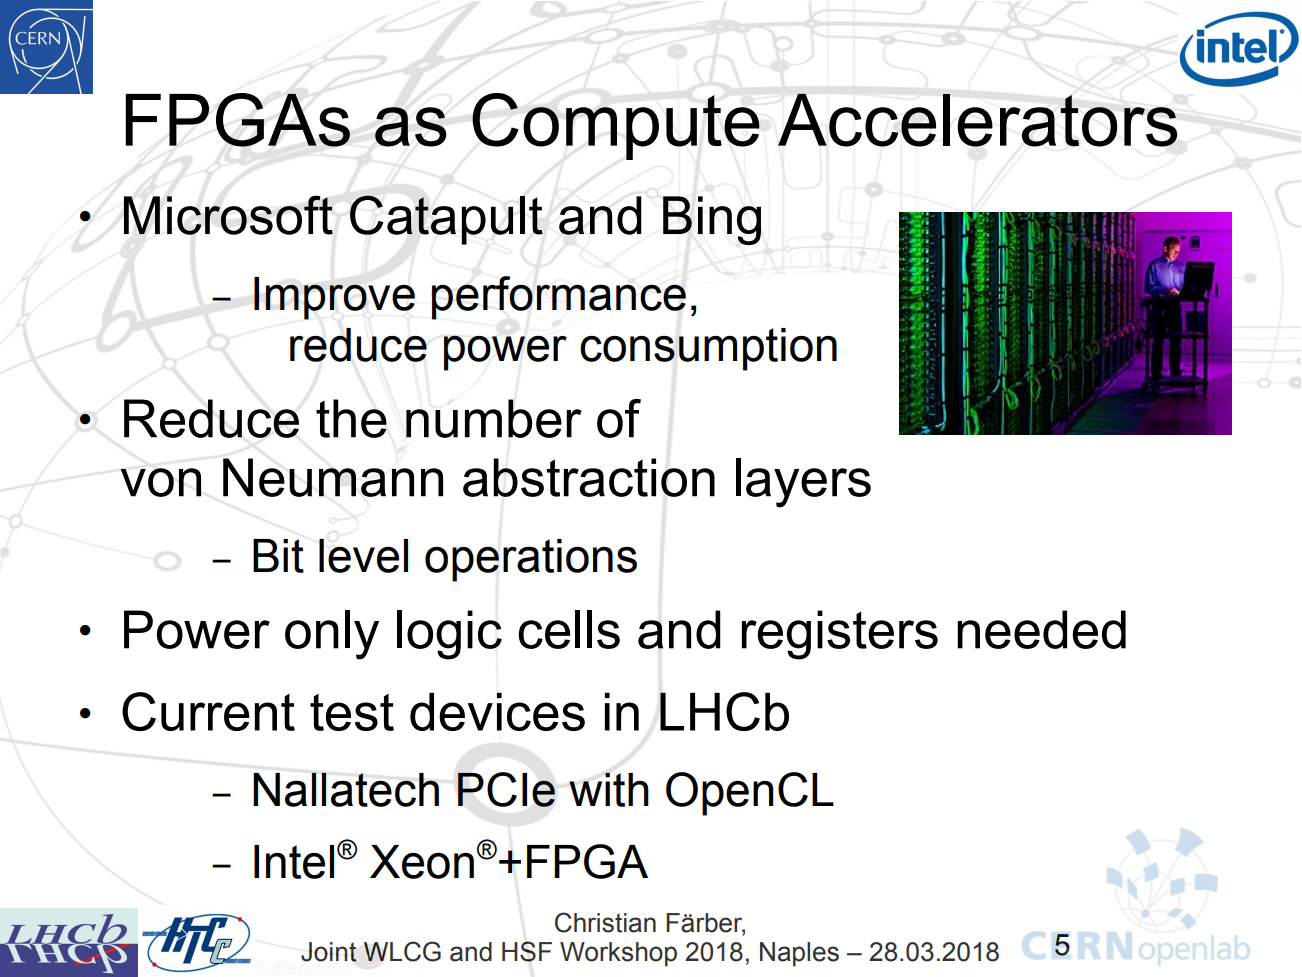
\includegraphics[width=0.73\linewidth]{fpgas-1.png}
\end{center}
\end{frame}

\begin{frame}{\textcolor{yellow}{\bf Christian Faerber:} FPGAs as co-processors for reconstruction}
\vspace{0.13 cm}
\begin{center}
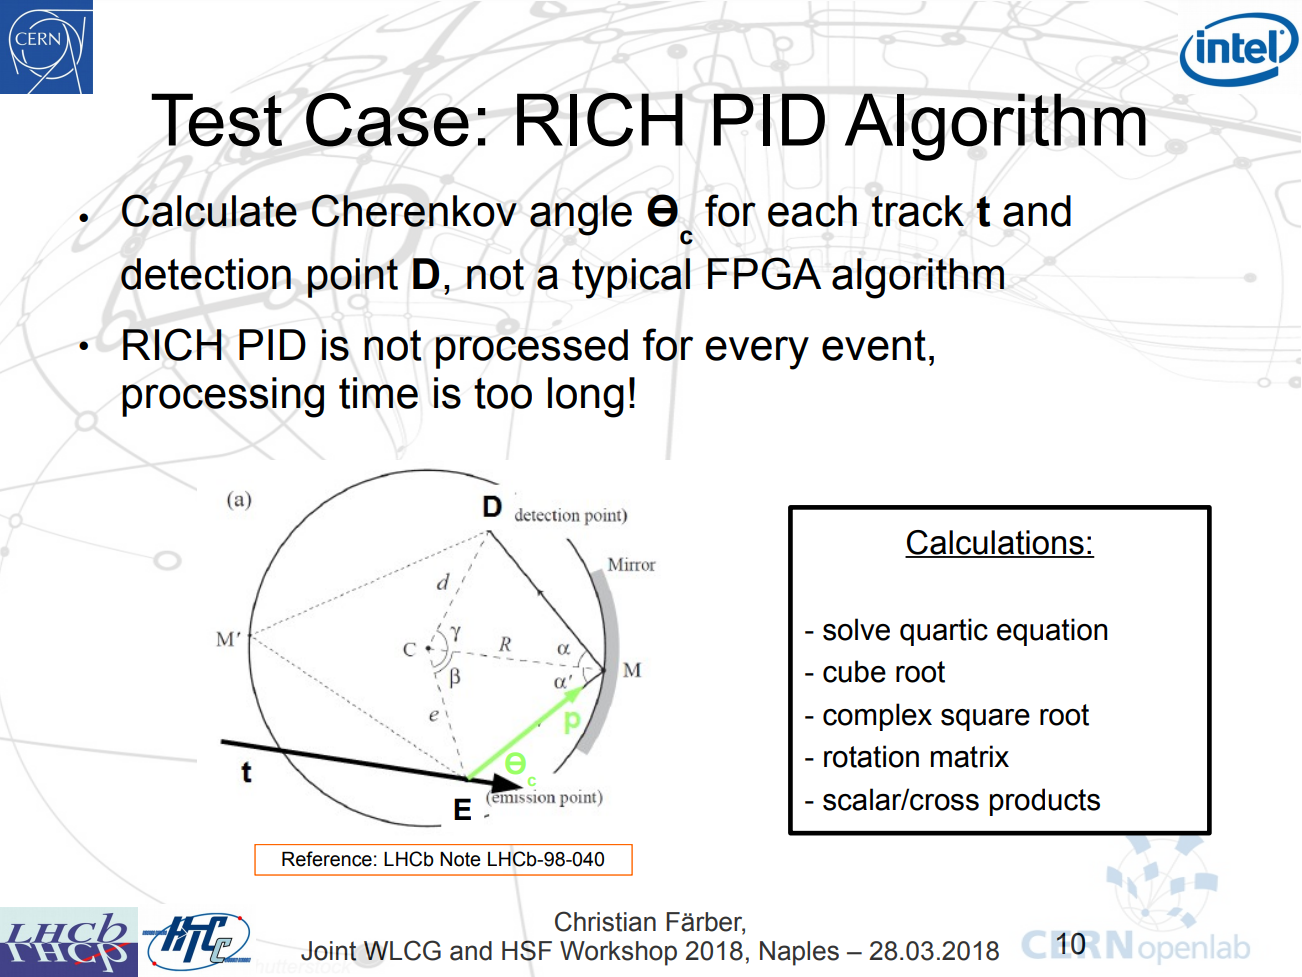
\includegraphics[width=0.73\linewidth]{fpgas-2.png}
\end{center}
\end{frame}

\begin{frame}{\textcolor{yellow}{\bf Christian Faerber:} FPGAs as co-processors for reconstruction}
\vspace{0.13 cm}
\begin{center}
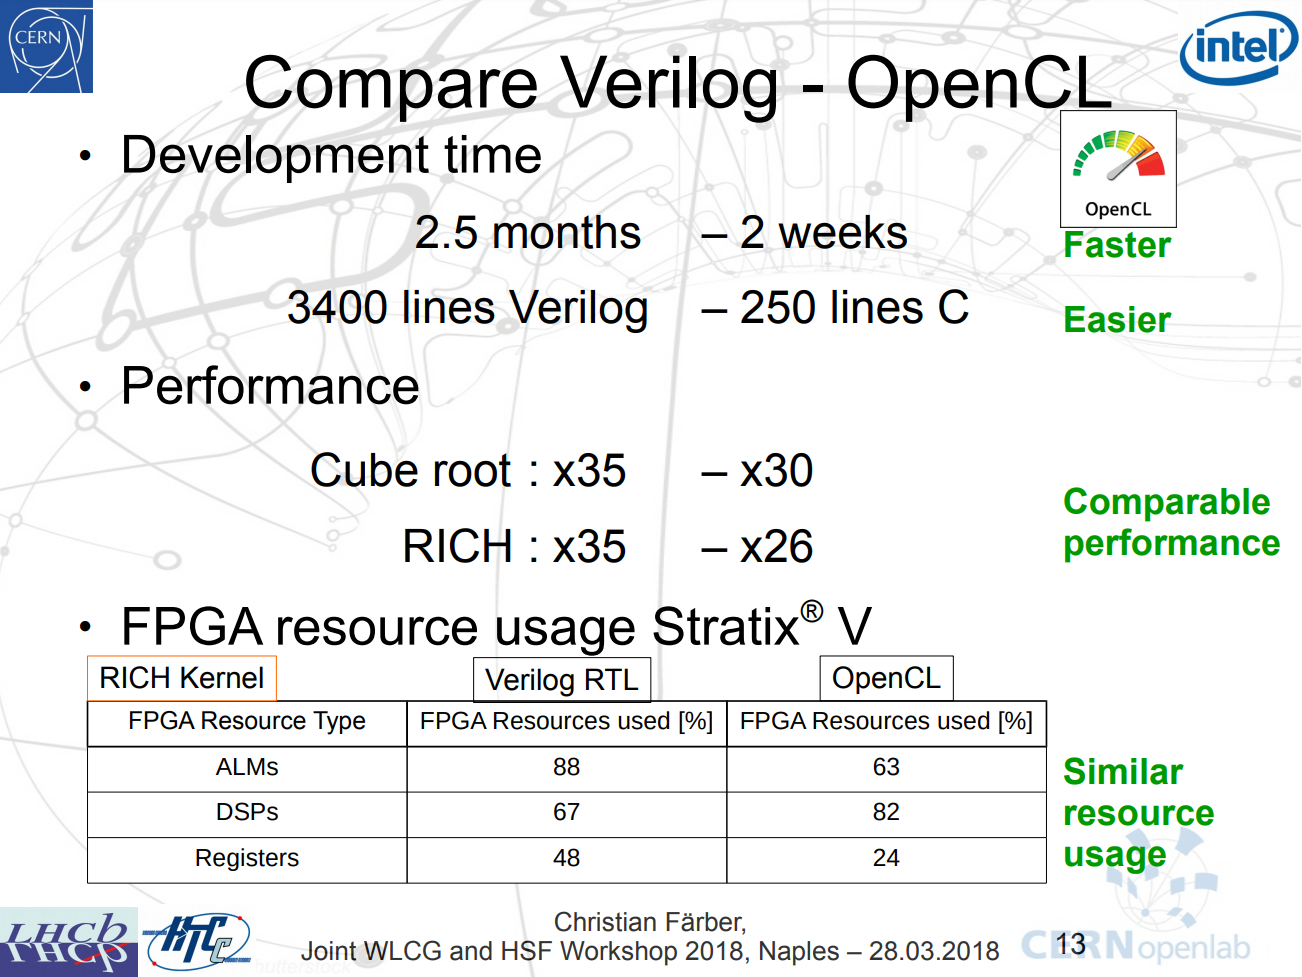
\includegraphics[width=0.73\linewidth]{fpgas-3.png}
\end{center}
\end{frame}

\begin{frame}{\textcolor{yellow}{\bf Andrei Gheata:} VecCore: Expressing HEP algos in explicit SIMD types}
\vspace{0.13 cm}
\begin{center}
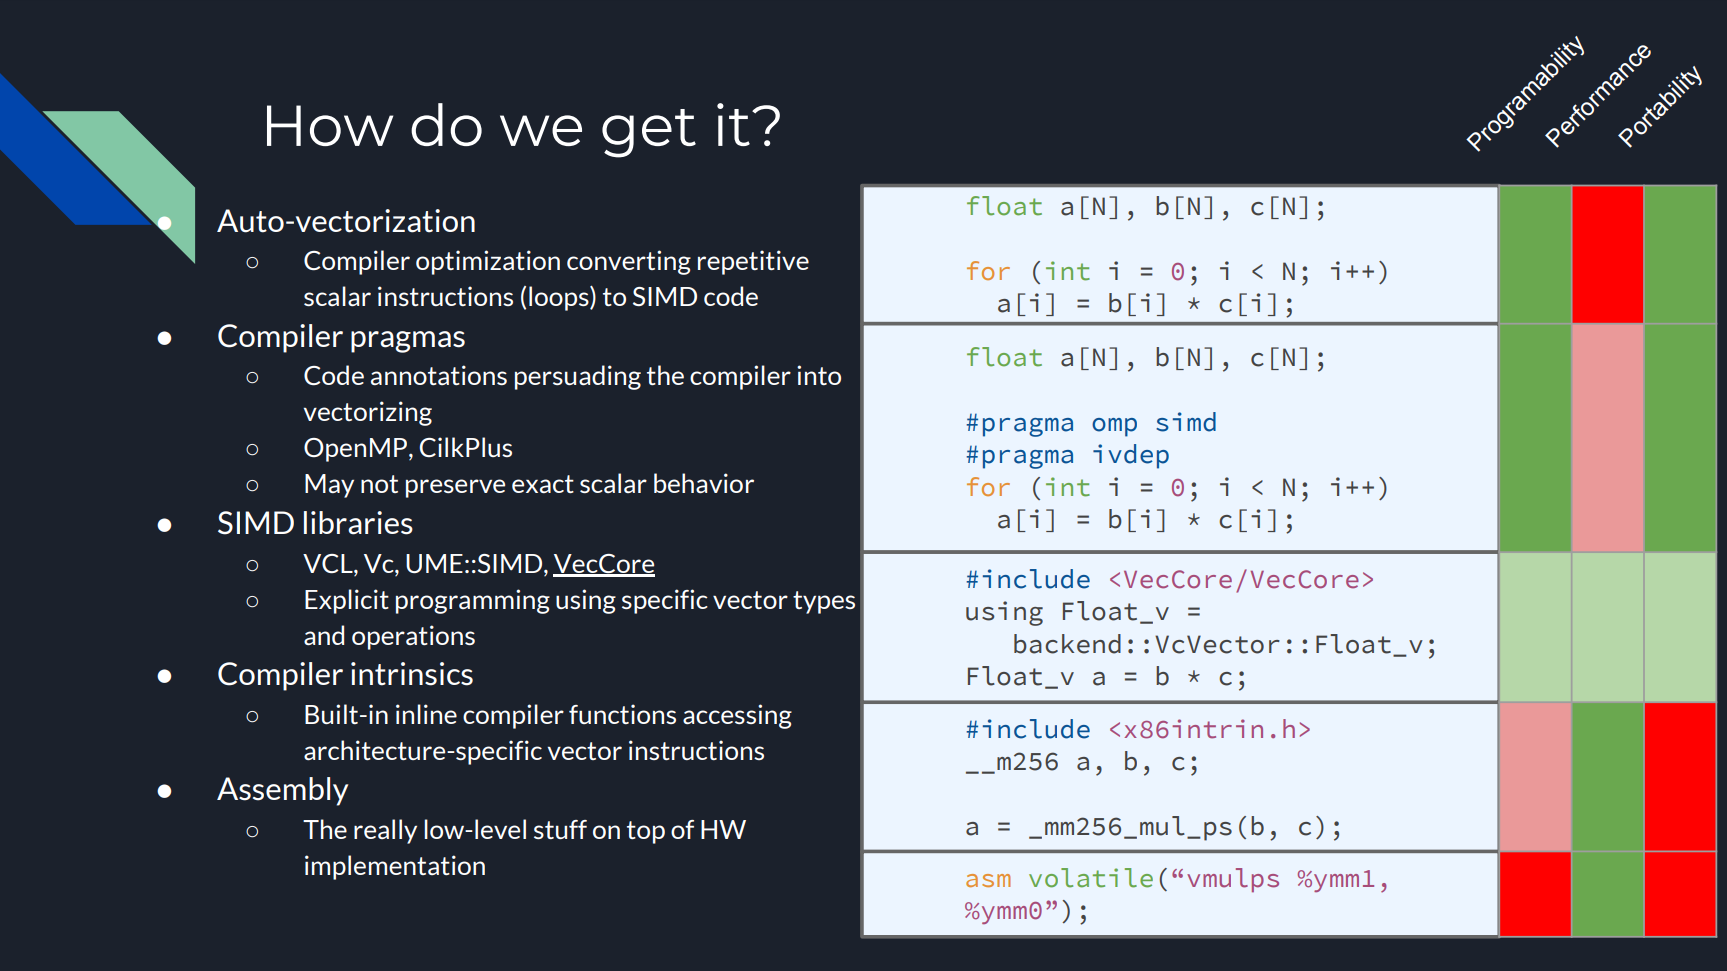
\includegraphics[width=0.95\linewidth]{veccore-1.png}
\end{center}
\end{frame}

\begin{frame}{\textcolor{yellow}{\bf Andrei Gheata:} VecCore: Expressing HEP algos in explicit SIMD types}
\vspace{0.13 cm}
\begin{center}
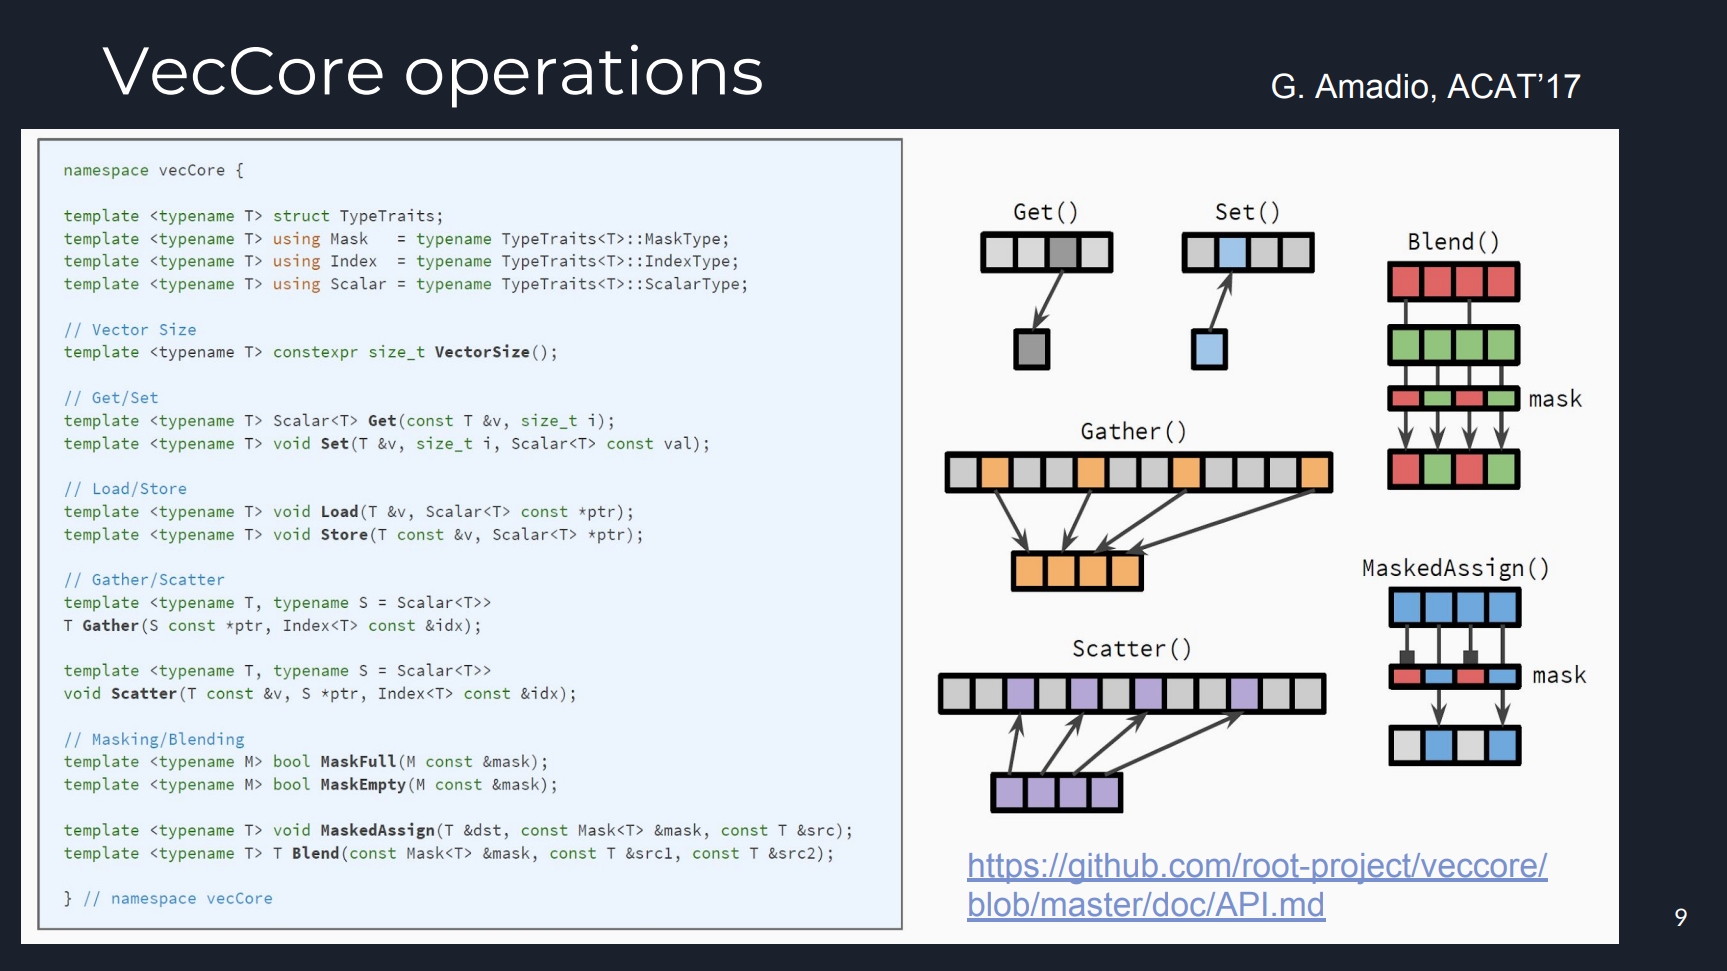
\includegraphics[width=0.95\linewidth]{veccore-2.png}
\end{center}
\end{frame}

\begin{frame}{\textcolor{yellow}{\bf Andrei Gheata:} VecCore: Expressing HEP algos in explicit SIMD types}
\vspace{0.13 cm}
\begin{center}
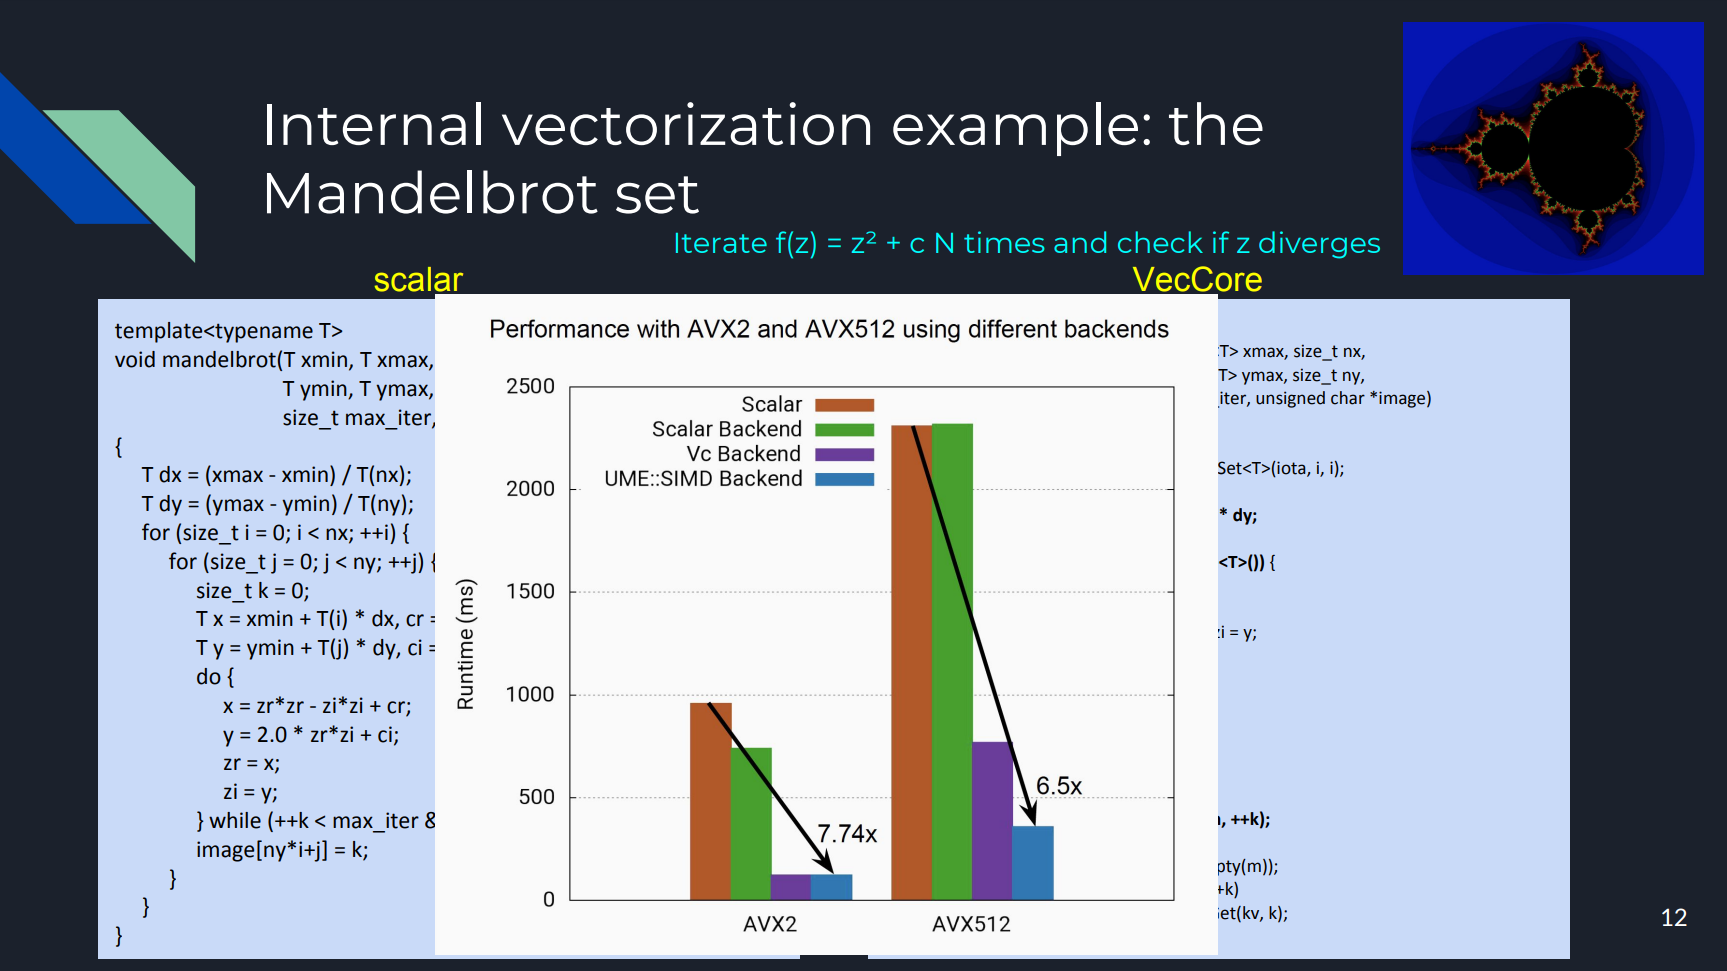
\includegraphics[width=0.95\linewidth]{veccore-3.png}
\end{center}
\end{frame}

\begin{frame}{\textcolor{yellow}{\bf Martin Durant:} Dask: distributed computing for scientific Python}
\vspace{0.13 cm}
\begin{center}
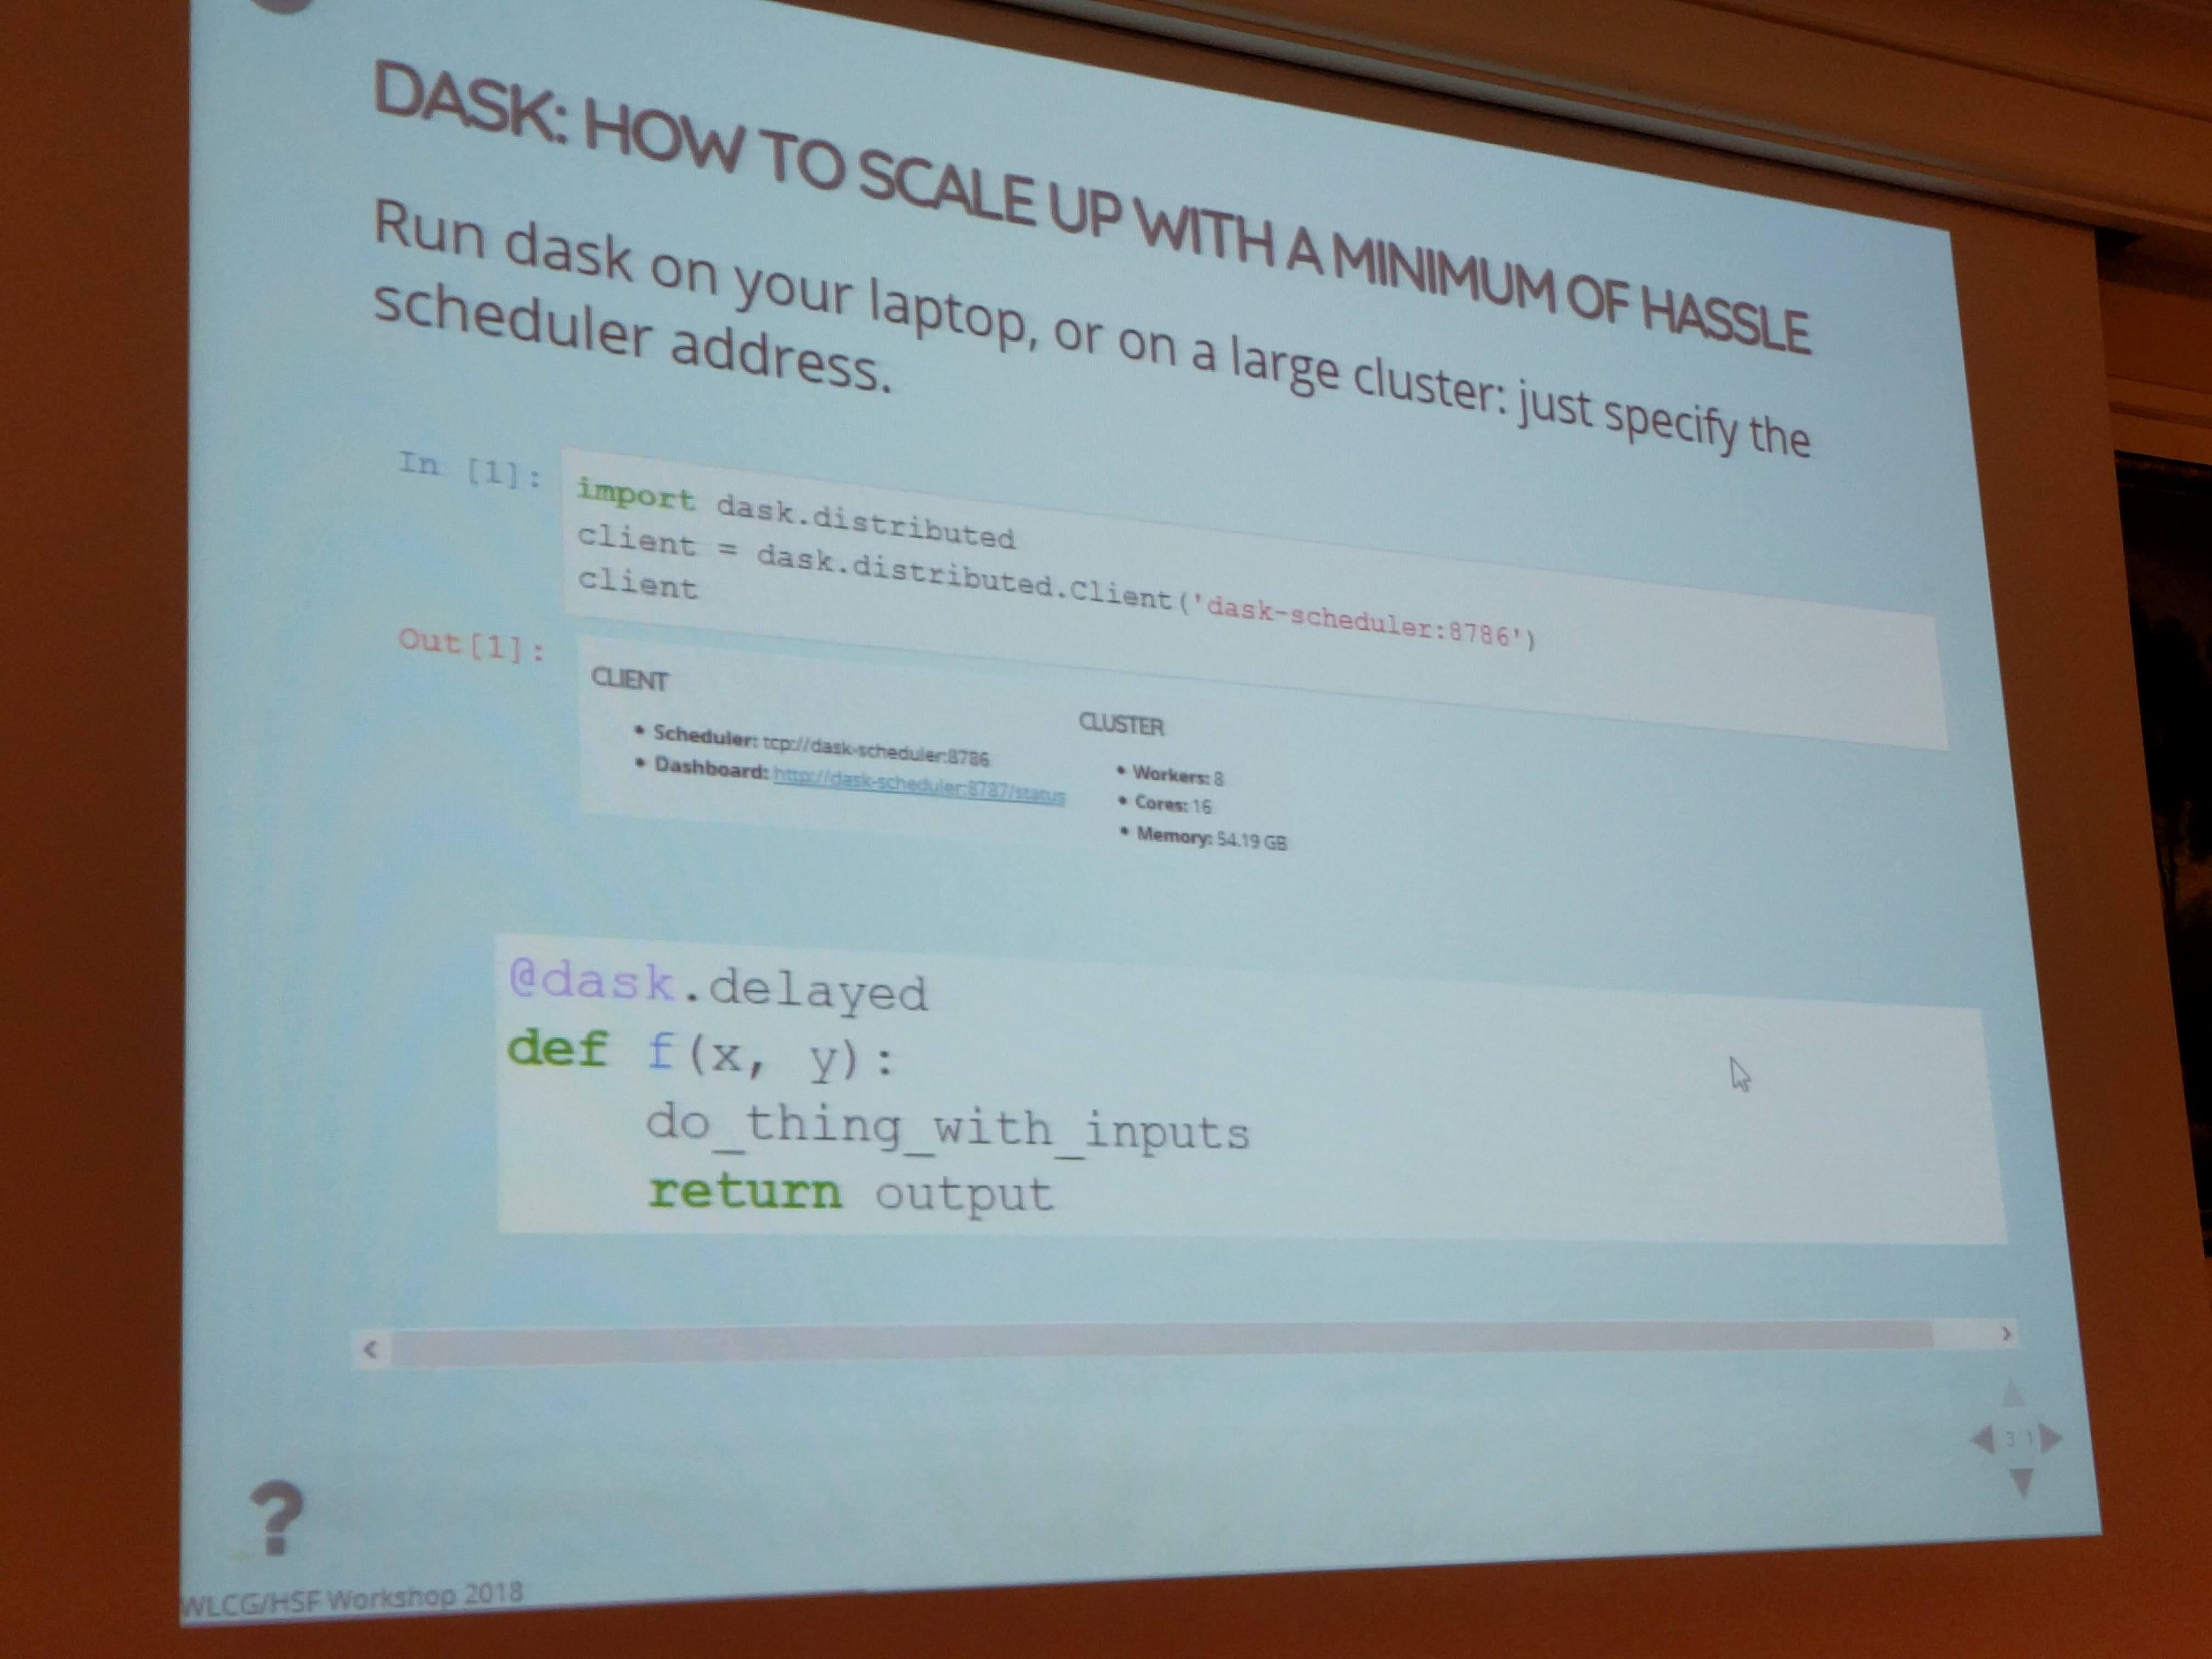
\includegraphics[width=0.73\linewidth]{dask-1.png}
\end{center}
\end{frame}

\begin{frame}{\textcolor{yellow}{\bf Martin Durant:} Dask: distributed computing for scientific Python}
\vspace{0.25 cm}
\includemedia[
  width=\linewidth,
  height=0.56\linewidth,
  activate=pageopen,
  addresource=dask-demo.mp4,
  flashvars={source=dask-demo.mp4}
]{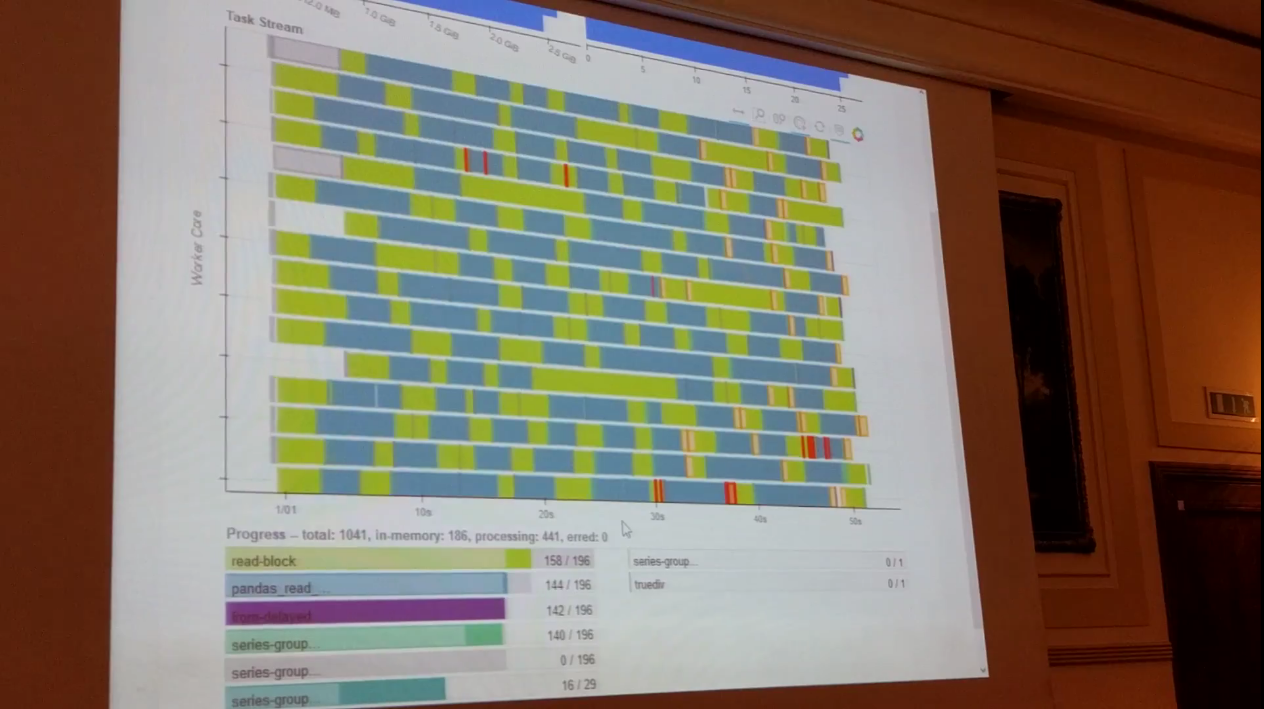
\includegraphics[width=\linewidth]{dask-demo-screenshot.png}}{VPlayer.swf}
\end{frame}

\begin{frame}{\textcolor{yellow}{\bf Martin Durant:} Dask: distributed computing for scientific Python}
\vspace{0.1 cm}
\begin{center}
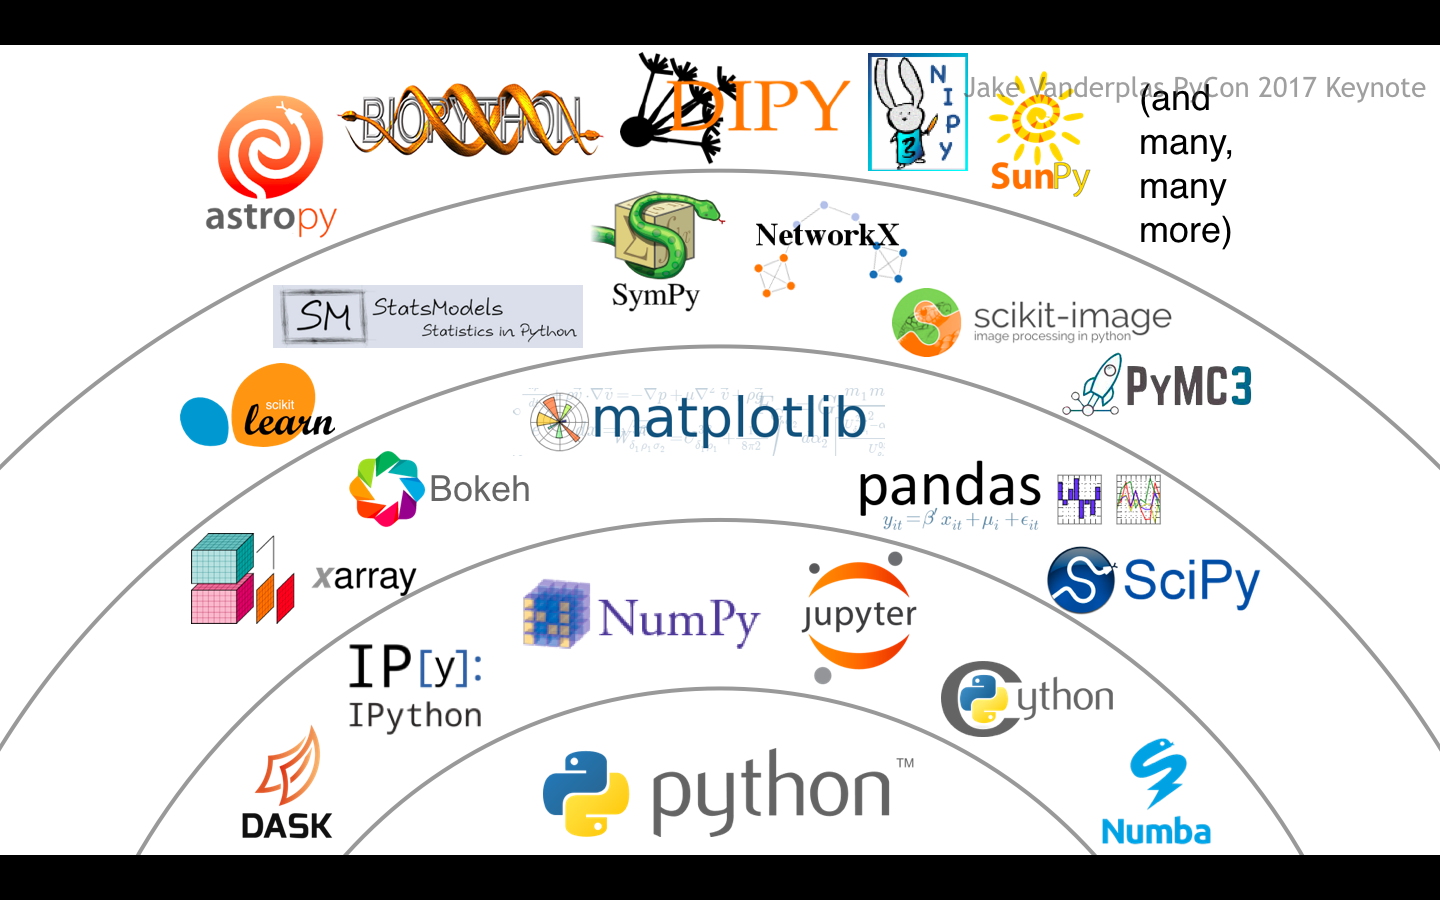
\includegraphics[width=0.88\linewidth]{dask-3.png}
\end{center}
\end{frame}

\begin{frame}{\textcolor{yellow}{\bf Matti Kortelainen:} Parallelized tracking algorithms}
\vspace{0.13 cm}
\begin{center}
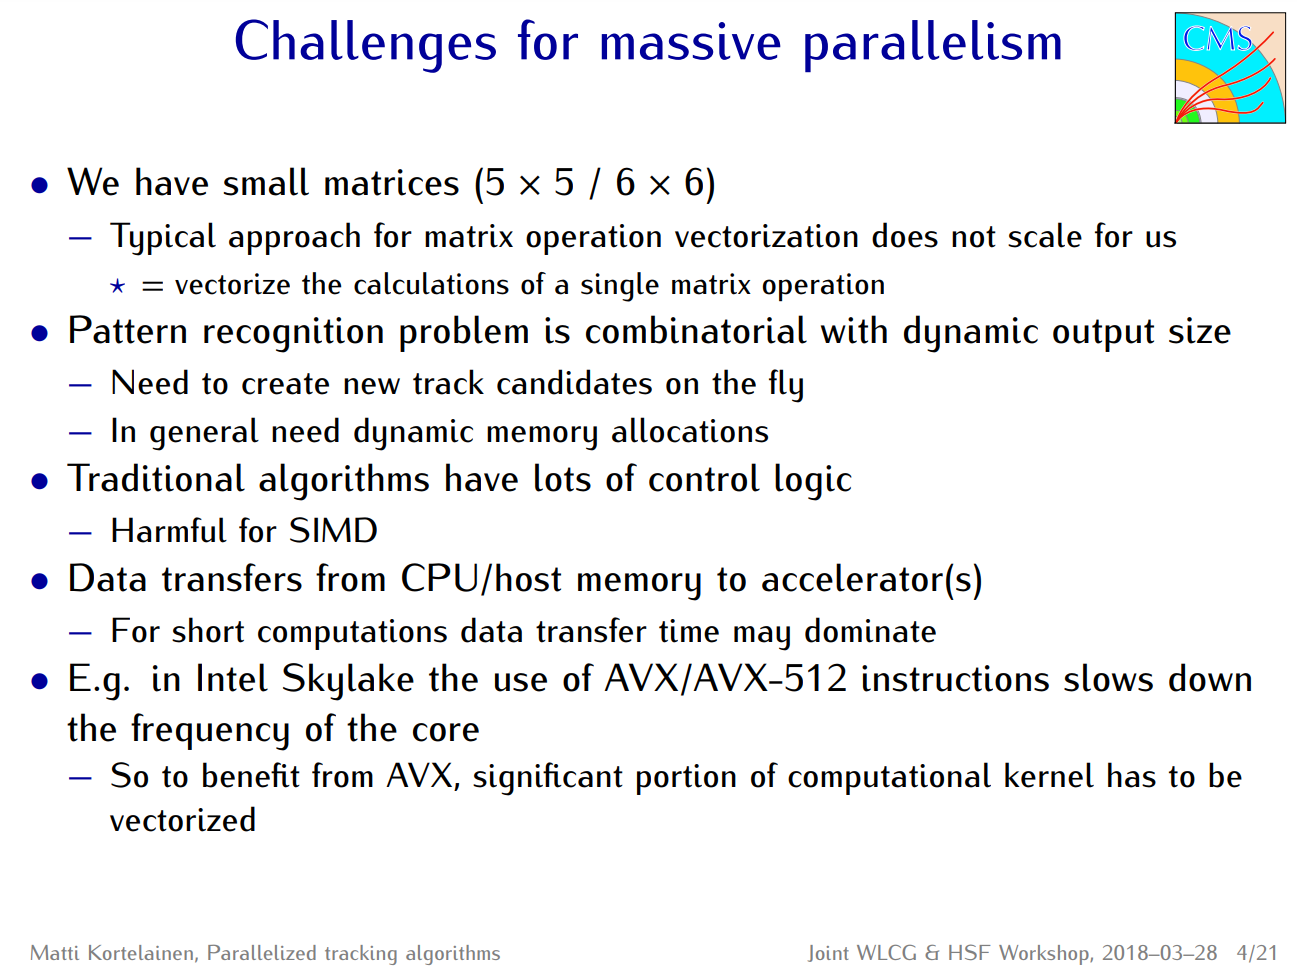
\includegraphics[width=0.73\linewidth]{tracking-1.png}
\end{center}
\end{frame}

\begin{frame}{\textcolor{yellow}{\bf Matti Kortelainen:} Parallelized tracking algorithms}
\vspace{0.13 cm}
\begin{center}
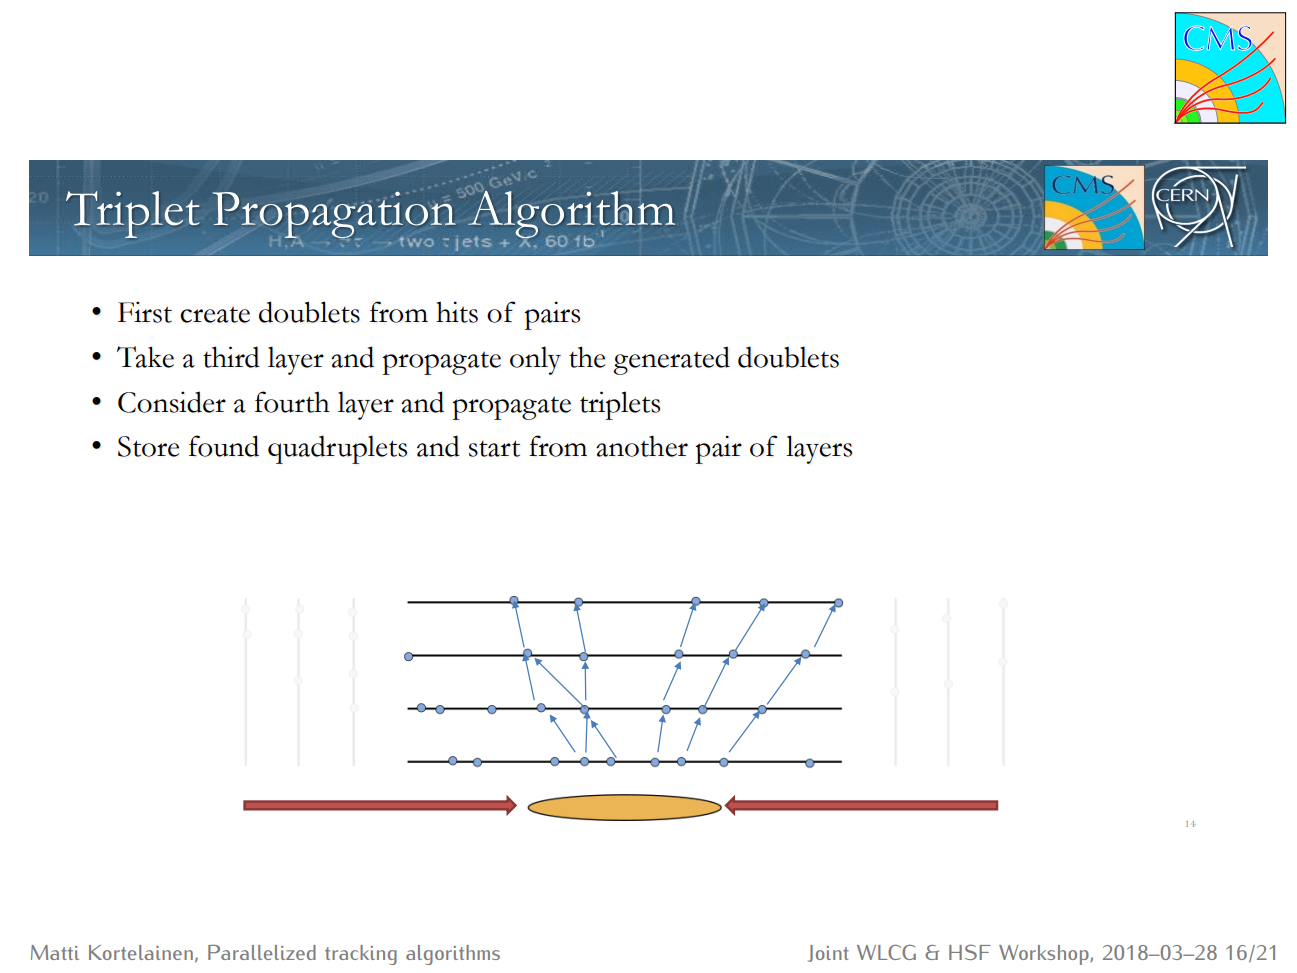
\includegraphics[width=0.73\linewidth]{tracking-2.png}
\end{center}
\end{frame}

\begin{frame}{\textcolor{yellow}{\bf Matti Kortelainen:} Parallelized tracking algorithms}
\vspace{0.13 cm}
\begin{center}
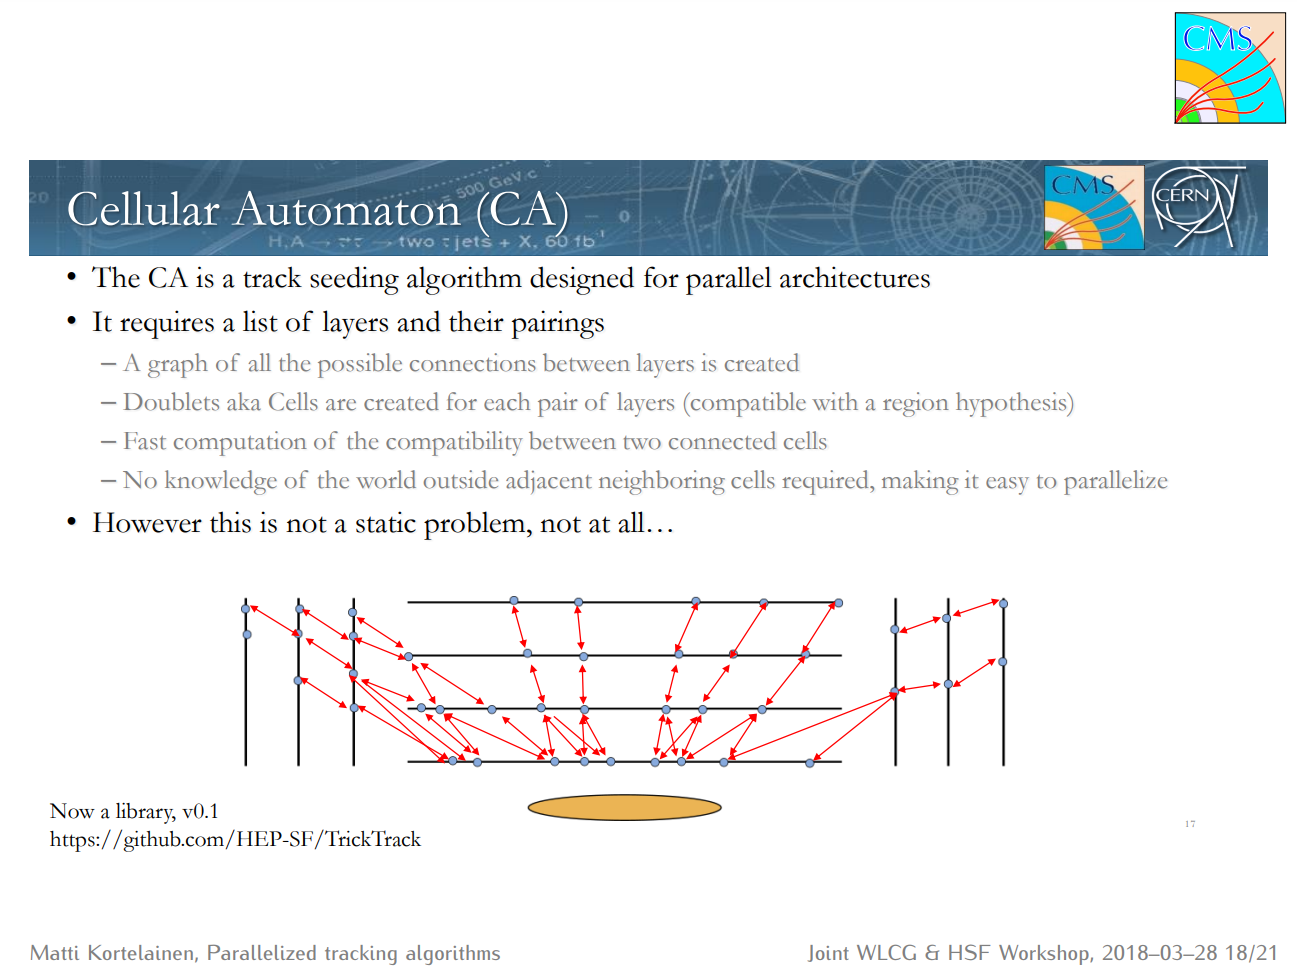
\includegraphics[width=0.73\linewidth]{tracking-3.png}
\end{center}
\end{frame}

\end{document}
